\section{AINEISTO}
    Keräsin tämän raportin aineiston Futuliigan lähetyksistä vuodelta 2023.
    Lähetyksiä oli yhteensä 23 ja niissä näytettiin heittoja 63 pelin 124 erästä.
    Lähetyksistä merkkasin niillä näkyvien heittojen aikaleimat ja ajat, jolloin konat saatiin pystyyn.
    Jokaisesta heitosta kirjasin myös heiton heittäjän.
    Heittojen kirjauksissa on varmasti yksittäisiä virheitä,
    mutta niiden vaikutus kokonaisanalyyseihin pitäisi olla pieni.
    Yhdestä heitosta puuttuva aika on lisätty toiseen heittoon,
    joten keskiarvoisesti heittojen kestot eivät ole muuttuneet.
    Yksittäisten pelaajien analyysiin virheilla on vaikutusta,
    varsinkin jos heittäjästä ei aineistossa ollut montaa heittoa.
    Heittäjien vertailu ei kuitenkaan ollut tämän analyysin tarkoitus,
    joten en ole käynyt aineistoa tarkemmin läpi.

    Sekä heittojen että konankasauksien aikaleimojen tarkkuus on sekunti.
    Johtuen muunmuassa videoiden joskus puutteellisesta tarkkuudesta,
    kamerakulmista johtuvista rajotteista
    ja YouTubessa satunnaisesti jäätyneestä videosta,
    aikaleimat eivät ole täysin tarkkoja.
    Heitoissa on pyritty merkitsemään aikaleimaksi se kuva, jolloin karttu on viimeisen kerran heittäjän kädessä.
    Konan katsoin kasatuksi, kun edellisessä erässä pelannut joukkue asetti viimeisen kyykän paikalleen tai viimeisen tornin kohdalleen.
    E\-si\-mer\-kik\-si peliä aloittamaan tulevan joukkueen tekemiä korjauksia en siis laskenut mukaan konankasausaikaan.

    Yksittäisten heittojen aikaleimoja kerättiin 3797 kappaletta ja konankasauksia 200 kappaletta.
    Analyysin kohteena oli heittäjän heittoon ja joukkueen konankasaamiseen käyttämän aika sekä pelien kesto,
    joten raakojen aikaleimojen sijaan analyysissa käytin niiden välisiä aikoja.
    Erän ensimmäisiin heittoihin kuluneet ajat laskin joko erä- tai pelitaukoon kuuluviksi,
    joten heittoaikoja oli loppujen lopuksi käytössä 3673 kappaletta.

    \begin{figure}[!ht]
        \centering
        \begin{subfigure}[b]{0.49\textwidth}
            \centering
            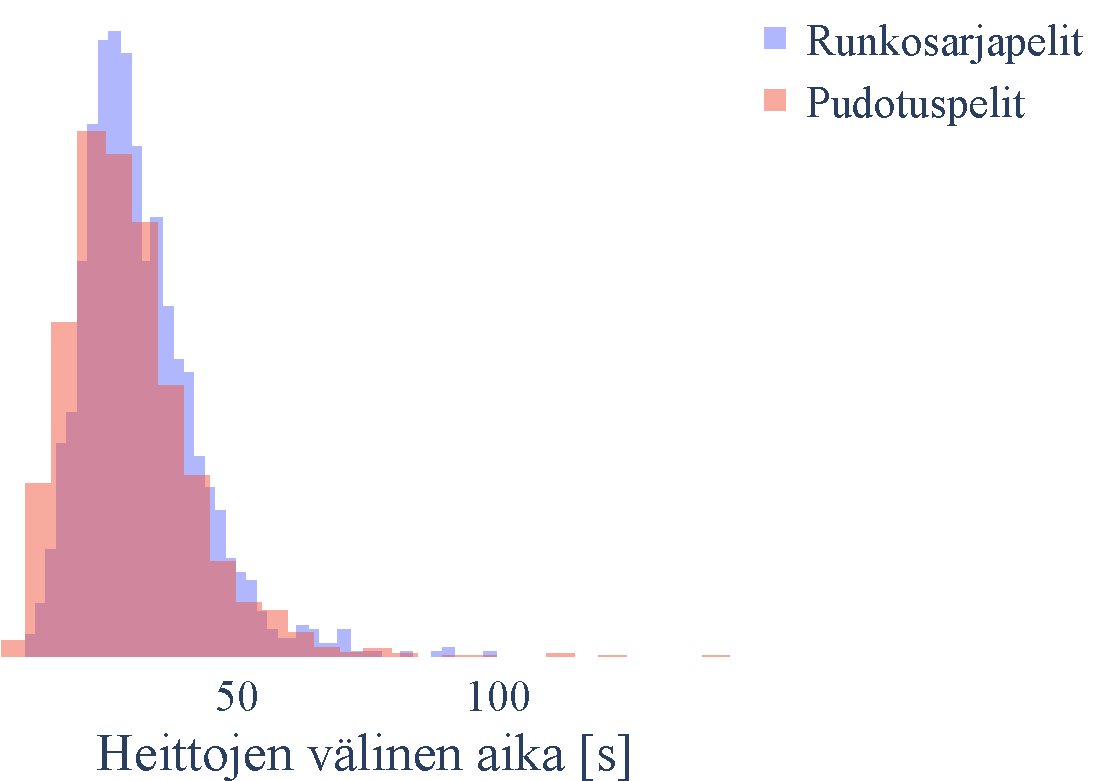
\includegraphics[width=\textwidth]{figures/heitot1.pdf}
            \caption{Runkosarjassa ja pudotuspeleissä\label{fig:throw_games}}
        \end{subfigure}
        \hfill
        \begin{subfigure}[b]{0.49\textwidth}
            \centering
            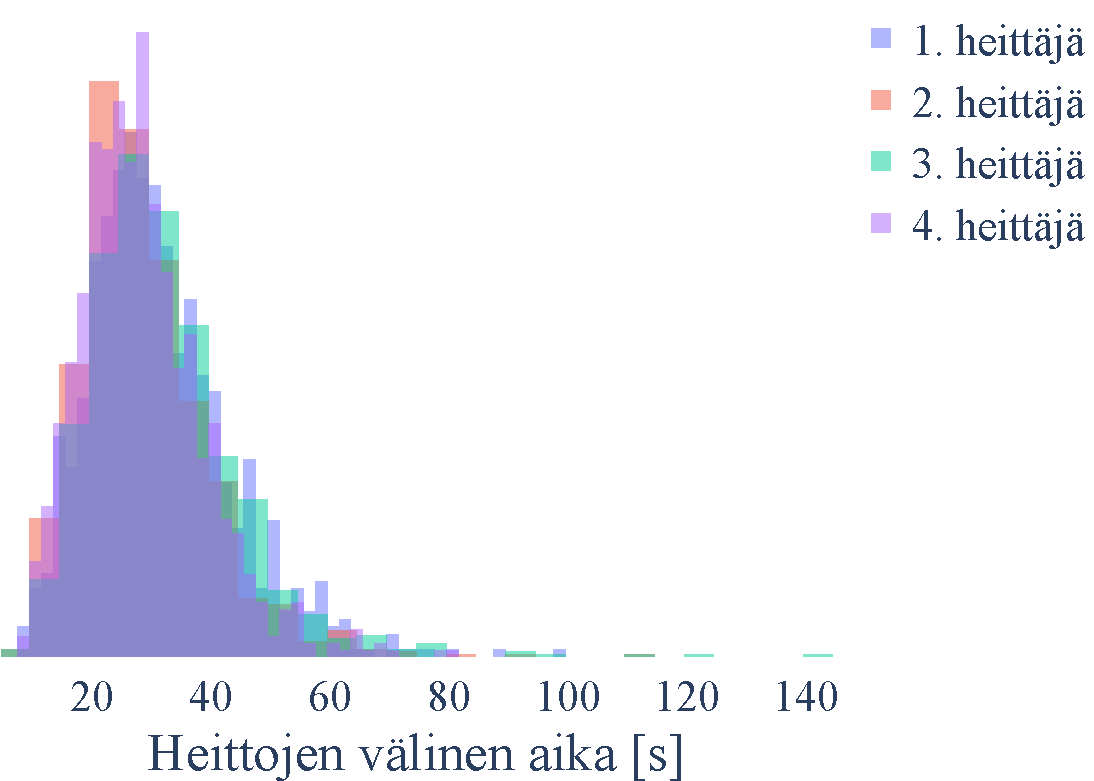
\includegraphics[width=\textwidth]{figures/heitot2.pdf}
            \caption{Heittopaikoittain\label{fig:throw_position}}
        \end{subfigure}
        \vspace{\baselineskip}
        \begin{subfigure}[b]{0.49\textwidth}
            \centering
            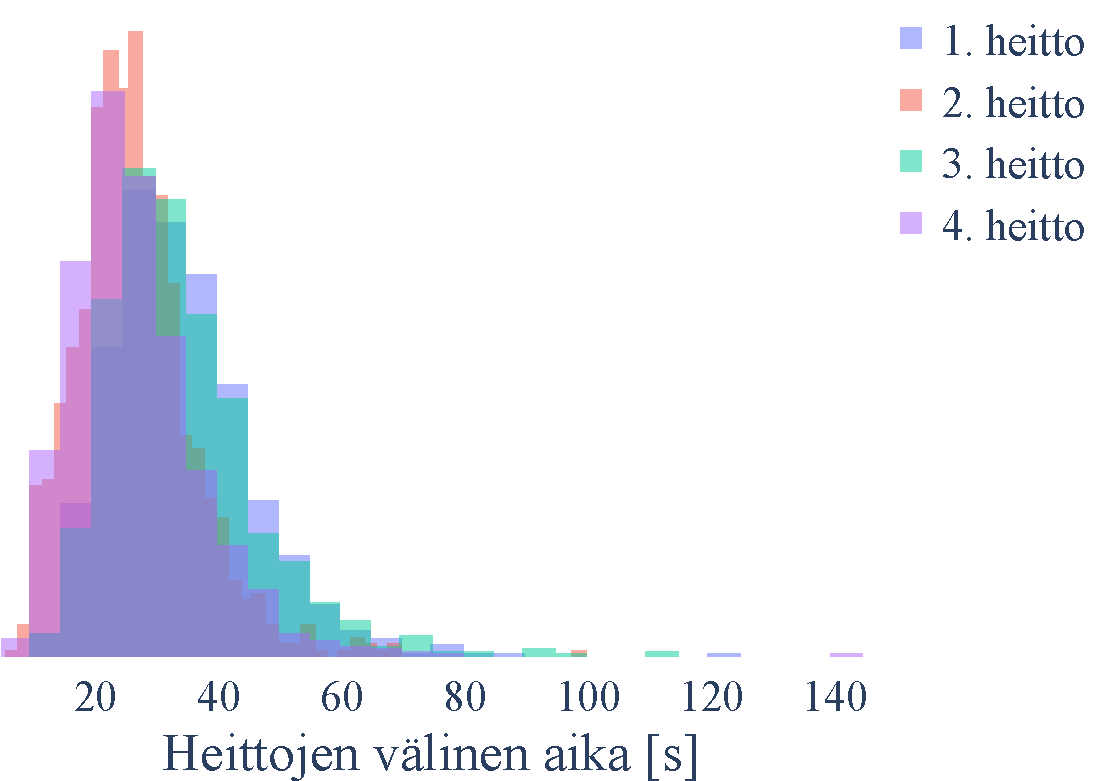
\includegraphics[width=\textwidth]{figures/heitot3.pdf}
            \caption{Heitoittain (per erä)\label{fig:throw}}
        \end{subfigure}
        \hfill
        \begin{subfigure}[b]{0.49\textwidth}
            \centering
            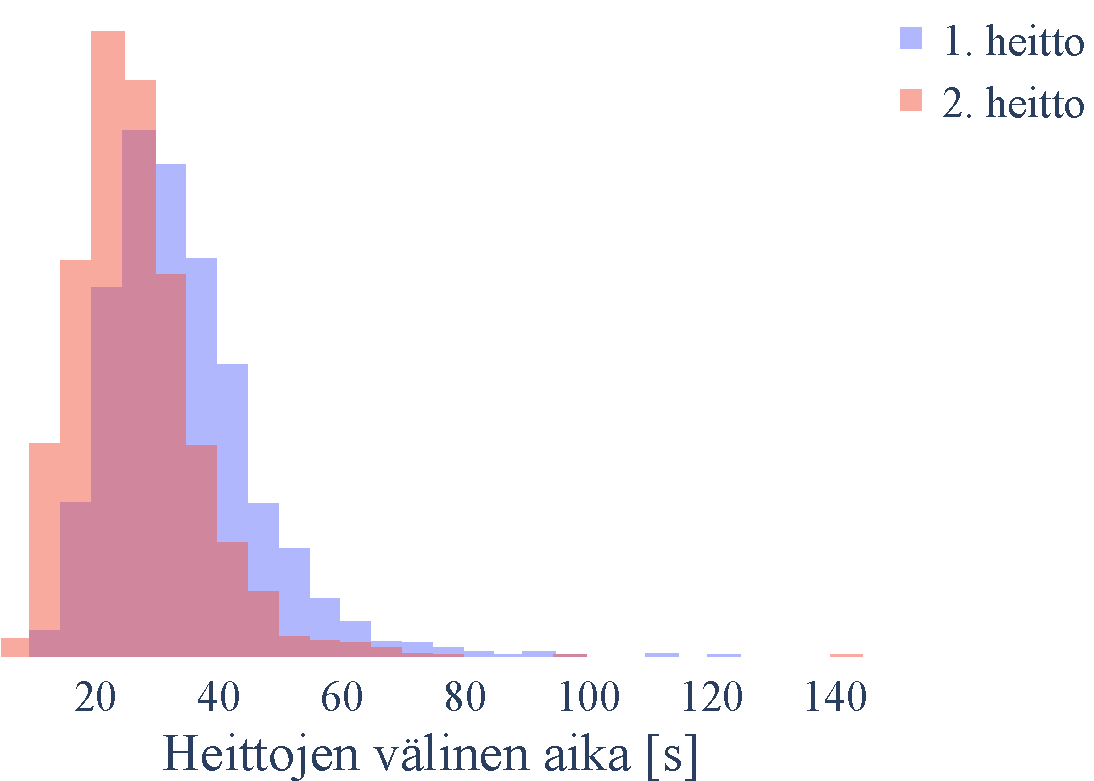
\includegraphics[width=\textwidth]{figures/heitot4.pdf}
            \caption{Heitoittain (per heittovuoro)\label{fig:throw2}}
        \end{subfigure}
        \caption{
            Heittoajan jakaumat.
            Yleisesti heittoaikojen jakauma ei ole symmetrinen vaan sillä on pitkä häntä oikealle.
            Visuaalisesti arvioituna heittoaikaan ei vaikuttanut, oliko peli runkosarjasta vai pudotuspeleistä,
            eikä se, monesko heittäjä heiton heitti.
            Erän ensimmäisen ja toisen puoliskon välillä ei myöskään vaikuttaisi olevan merkittävää vaikutusta.
            Sen sijaan pelaajan ensimmäisen ja toisen heiton välinen ero oli selkeä.\label{fig:throws}
        }
    \end{figure}

    Heittoaikoja on esitelty \fref{kuvassa}{fig:throws}
    ja niiden keskiarvoja \fref{taulukossa}{tab:averages}.
    Kuten asioiden kestojen jakaumat usein ovat, on heittoaikojen jakauma epäsymmetrinen.
    Nopein heitto heitettiin 7 sekunnissa ja hitaimpaan käytetiin 2 minuuttia ja 22 sekuntia.
    Pisimmät yksittäiset heittojat liittyvät joko vaikeiden tilanteiden tai pappien pohtimiseen.
    Heiton kestoon vaikuttavista syistä esiin nousi heittovuoron ensimmäiseen heittoon käytetty aika.
    Luultavasti tämä ero johtuu heittovälineiden keräilyyn ja neliöön siirtymiseen käytetystä ajasta.

    \begin{figure}[!ht]
        \centering
        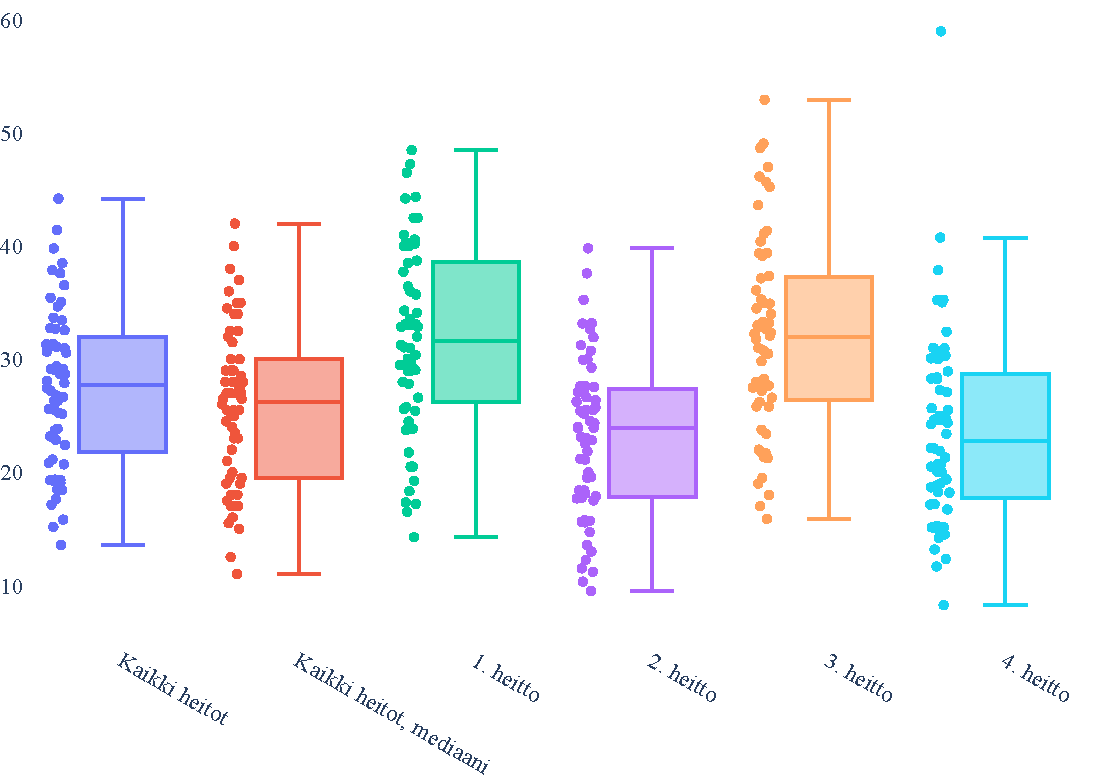
\includegraphics[width=\textwidth]{figures/keskiarvot1.pdf}
        \caption{
            Pelaajien keskimääräiset heittoajat.
            Heittoaikojen keskiarvojen ja mediaanien ero ei ole suuri verrattuna pelaajien välisiin vaihteluihin.
            Heittovuoron ensimmäisen ja toisen heiton välillä on selkeä ero heiton kestossa,
            mutta heitot eivät näyttäisi hidastuvan pelin edetessä.\label{fig:players}
        }
    \end{figure}
    \begin{figure}[!ht]
        \centering
        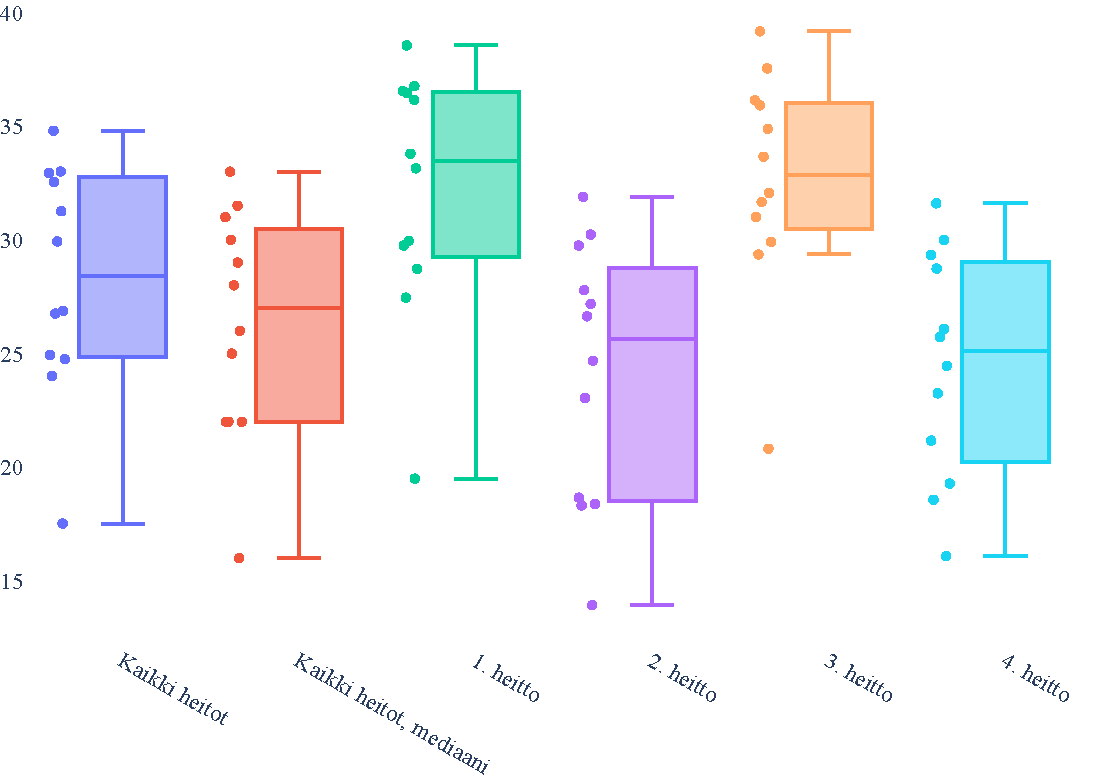
\includegraphics[width=\textwidth]{figures/keskiarvot2.pdf}
        \caption{
            Joukkueiden keskimääräiset heittoajat.
            Kuvassa näkyvät ilmiöt ovat hyvin samankaltaisia kuin \fref{kuvassa}{fig:players}.\label{fig:teams}
        }
    \end{figure}

    Pelaajien ja joukkueiden keskimääräiset heittoajat näkyvät \fref{kuvissa}{fig:players} \fref{ja}{fig:teams}.
    Keskiarvoissa on suurehkoa vaihtelua,
    mutta niiden jakaumassa ei ole nähtävissä samanlaista pitkää häntää kuin yksittäisten heittojen jakaumassa,
    mikäli pienestä otoksesta johtuva, noin minuutin keskiarvo neljännelle heitolle jätetään huomiotta.
    Keskiarvojen jakaumat ovat jotakuinkin symmetrisiä eikä keskiarvojen ja mediaanien välillä ole suurta eroa,
    joten yksittäisten kauan kestäneiden heittojen vaikutus keskiarvoihin lienee pieni.
    Heittojen välisiä keskiarvoja vertaillessa voi huomata saman kuin yksittäisten heittojen jakaumista:
    erän ensimmäisten ja toisten heittojen välillä ei ole merkittävää eroa,
    mutta heittovuorossa ensimmäinen heitto on usein toista heittoa hitaampi.  

    \begin{figure}[!ht]
       \centering
       \begin{subfigure}[b]{0.4\textwidth}
           \centering
           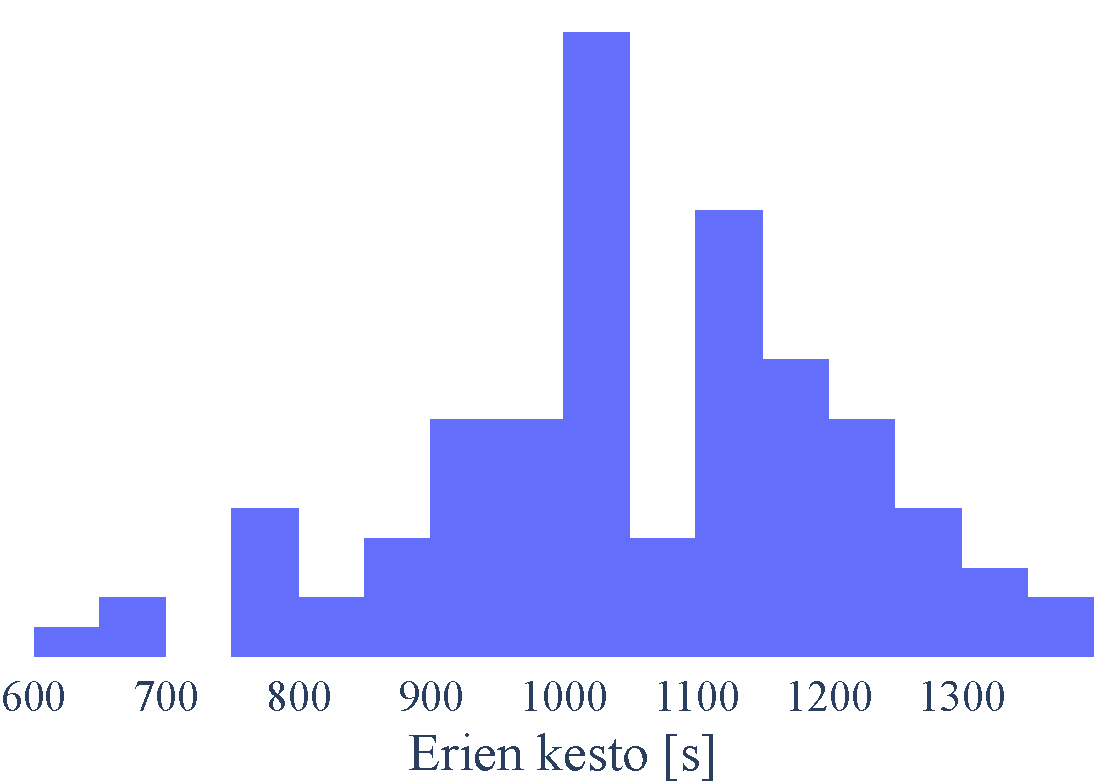
\includegraphics[width=\textwidth]{figures/pelit1.pdf}
       \end{subfigure}
       \hfill
       \begin{subfigure}[b]{0.4\textwidth}
           \centering
           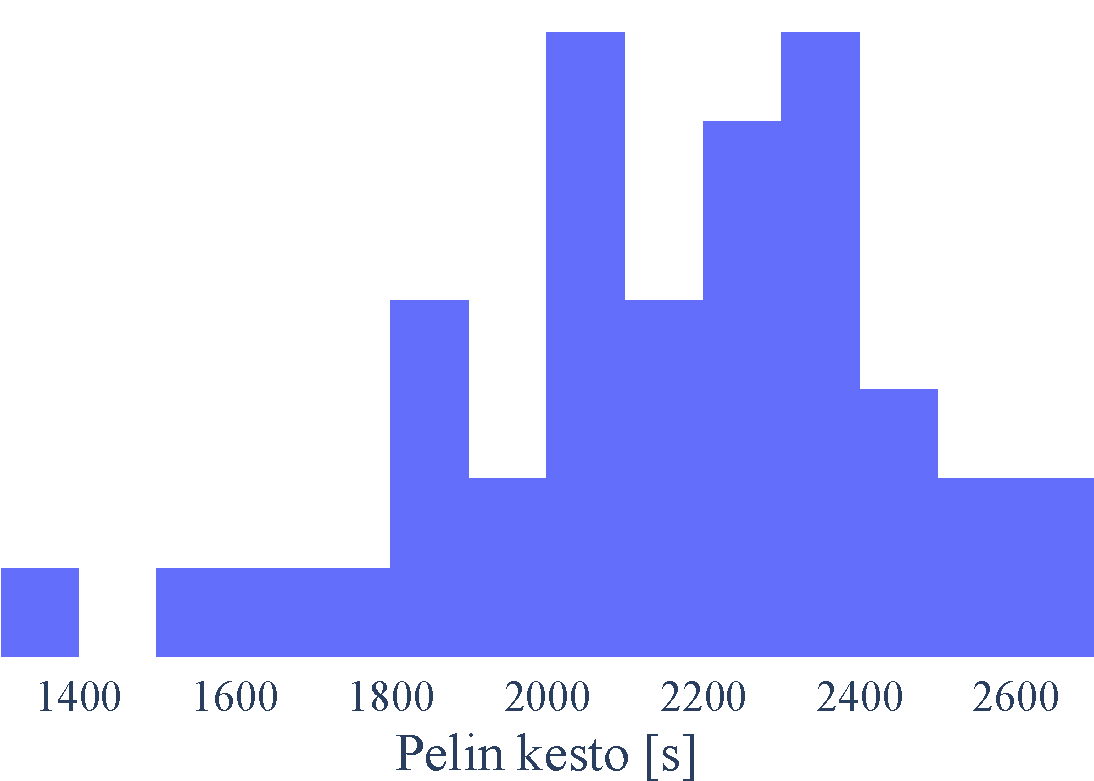
\includegraphics[width=\textwidth]{figures/pelit2.pdf}
       \end{subfigure}
       \vspace{\baselineskip}
       \begin{subfigure}[b]{0.4\textwidth}
           \centering
           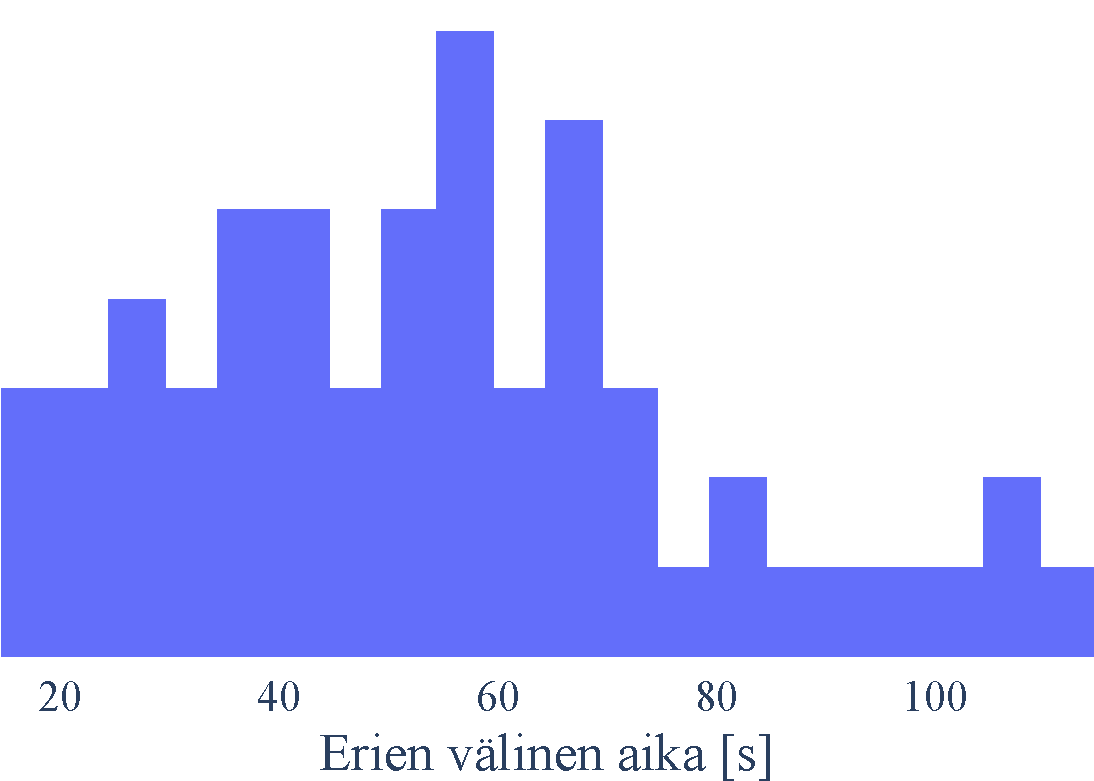
\includegraphics[width=\textwidth]{figures/pelit3.pdf}
       \end{subfigure}
       \hfill
       \begin{subfigure}[b]{0.4\textwidth}
           \centering
           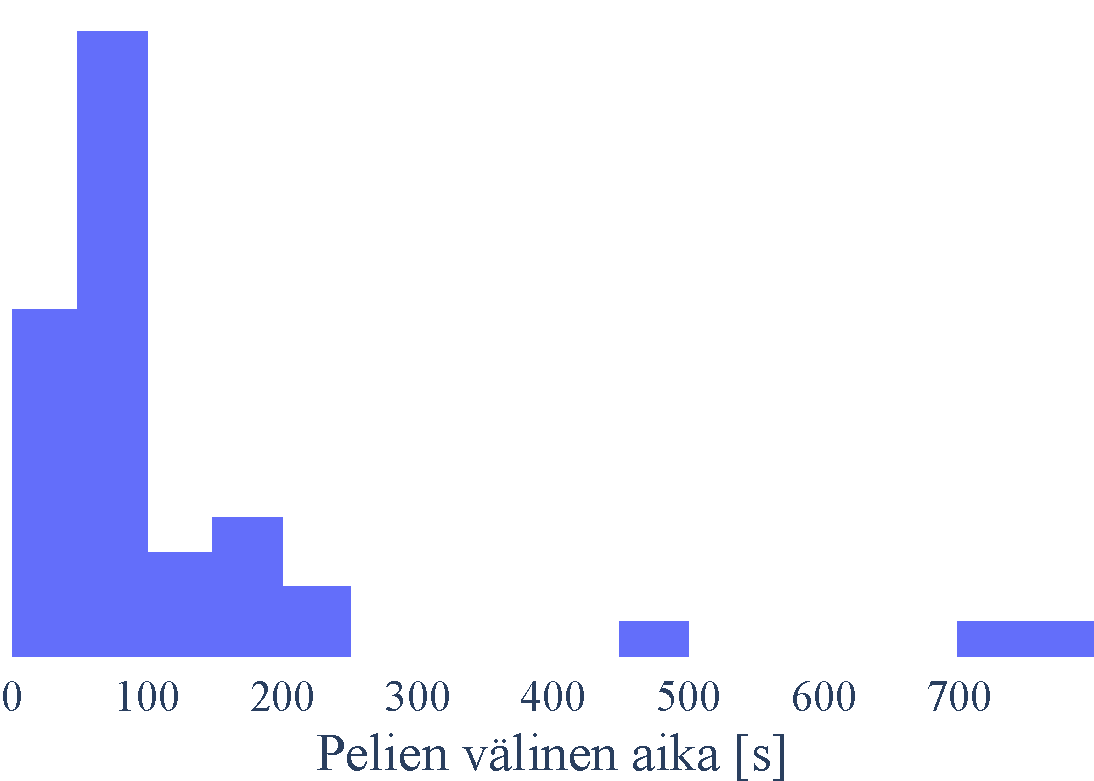
\includegraphics[width=\textwidth]{figures/pelit4.pdf}
       \end{subfigure}
       \caption{
        Pelien kestojen jakaumat.
        Erien ja pelien kestot ovat jakautuneet lähes symmetrisesti.
        Huomattavaa on, että pisin erä kesti lähes yhtäpitkään kuin lyhyin peli.
        Erätauot ovat hyvin tasaisesti jakautuneita eikä pisinkään tauko ollut kauhean pitkä,
        mutta osa pelitauoista kesti yli kymmenen minuuttia.\label{fig:games}
        }
    \end{figure}
   
    Pelien kestoon vaikuttavia aikoja on esitelty \fref{kuvassa}{fig:games}
    ja niiden keskiarvoja \fref{taulukossa}{tab:averages}.
    Keskiarvoihin ja kuviin on käytetty vain pelejä, jotka näkyivät lähetyksissä kokonaan.
    Niissä peleissä, jotka olivat lähetysten viimeisiä, ei ole mukana konankasauksia.
    Lisäksi pelitaukojen tulkinnassa kannattaa huomioida,
    että osa tauoista on venynyt odotellessa viereisen kentän pelin loppumista.

    Erien ja pelien kestojen jakaumat ovat lähes symmetrisiä,
    mutta varsinkin pelitauoissa on nähtävissä samanlainen häntä kuin heittoaikojenkin jakaumassa.
    Koska kaikista otteluista ei tallennettu molempia eriä,
    kahden erän ja yhden erätauon keskimääräinen kesto ei täsmää ottelun keskimääräisen keston kanssa.
    Keskimääräinen ottelu oli pidempi kuin \fref{taulukossa}{tab:averages} on esitetty.
    Nopein erä kesti 10 minuuttia ja 4 sekuntia ja nopein ottelu 22 minuuttia ja 21 sekuntia.
    Pisimpään erään ja otteluun taasen käytettiin 22 minuuttia 47 sekuntia ja 44 minuuttia 45 sekuntia.

    \begin{figure}[!ht]
        \centering
        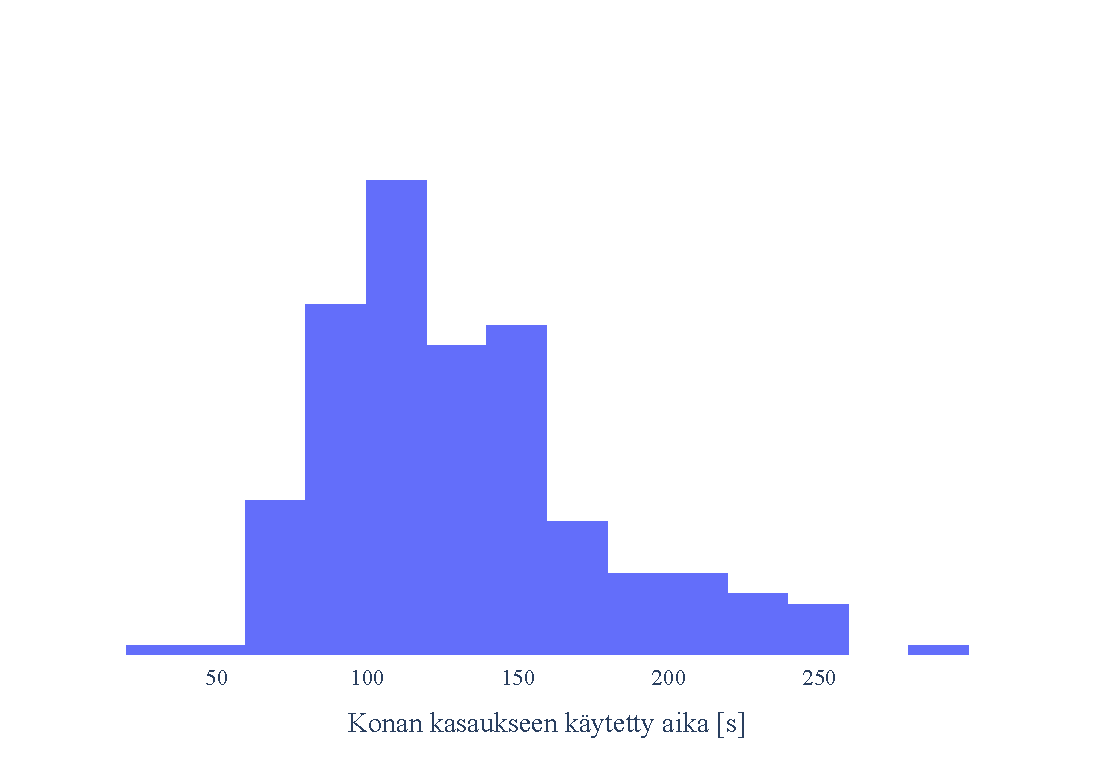
\includegraphics[width=\textwidth]{figures/konat.pdf}
        \caption{Konankasausaikojen jakauma\label{fig:konat}}
    \end{figure}

    Konankasaukseen käytetyn ajan (\fref{Kuva}{fig:konat}) jakauma on epäsymmetrinen kuten heittoaikojen jakauma.
    Kasausaikojen vaihtelu on maltillista, eikä merkittävästi keskiarvosta poikkeavia arvoja ole.

    \begin{table}[!ht]
        \centering
        \begin{tabular}{@{}lr@{}}
            \toprule
            Tapahtuma & Keskimääräinen kesto \\
            \midrule
            Heitto & 30,1 s \\
            Ensimmäisen ja toisen heiton ero & 7,5 s \\
            Konan kasaaminen & 2 min 11 s \\
            Erä & 17 min 35 s \\
            Peli & 35 min 54 s \\
            Erätauko & 54,6 s \\
            Pelitauko & 2 min 14 s \\
            \bottomrule
        \end{tabular}
        \caption{Aineiston keskiarvoja\label{tab:averages}}
    \end{table}